\begin{figure*}[p]
\centering
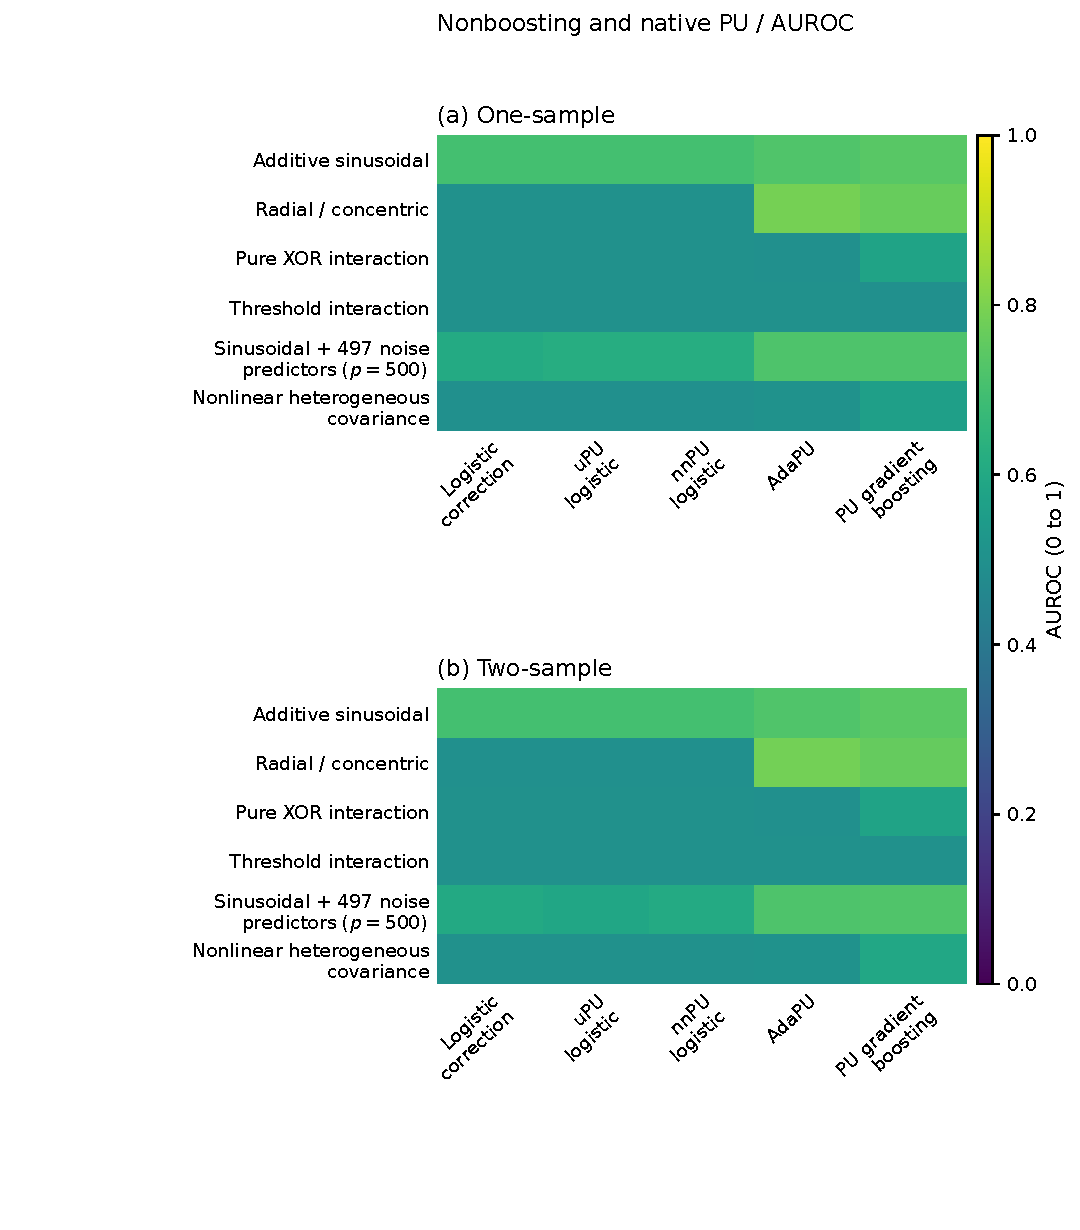
\includegraphics[page=1,width=\textwidth]{revised_figures/fig_s_nonlinear_full.pdf}
\caption{All 25 nonlinear-extension PU configurations, separated into prespecified method blocks. AUROC and AP use final train+validation refits. Individual DGPs are primary, and scales are fixed at 0 to 1. Six unavailable RN refits remain missing; asterisks mark means based on 99 rather than 100 successful refits. Nonboosting and native PU / AUROC. All six nonlinear DGPs. * n=99; all other cells n=100. Missing refits are not imputed.}
\label{fig:s-nonlinear-full-1}
\end{figure*}
\begin{figure*}[p]
\centering
\includegraphics[page=2,width=\textwidth]{revised_figures/fig_s_nonlinear_full.pdf}
\caption{All 25 nonlinear-extension PU configurations, separated into prespecified method blocks. AUROC and AP use final train+validation refits. Individual DGPs are primary, and scales are fixed at 0 to 1. Six unavailable RN refits remain missing; asterisks mark means based on 99 rather than 100 successful refits. Naive boosting / AUROC. All six nonlinear DGPs. * n=99; all other cells n=100. Missing refits are not imputed.}
\label{fig:s-nonlinear-full-2}
\end{figure*}
\begin{figure*}[p]
\centering
\includegraphics[page=3,width=\textwidth]{revised_figures/fig_s_nonlinear_full.pdf}
\caption{All 25 nonlinear-extension PU configurations, separated into prespecified method blocks. AUROC and AP use final train+validation refits. Individual DGPs are primary, and scales are fixed at 0 to 1. Six unavailable RN refits remain missing; asterisks mark means based on 99 rather than 100 successful refits. Corrected boosting / AUROC. All six nonlinear DGPs. * n=99; all other cells n=100. Missing refits are not imputed.}
\label{fig:s-nonlinear-full-3}
\end{figure*}
\begin{figure*}[p]
\centering
\includegraphics[page=4,width=\textwidth]{revised_figures/fig_s_nonlinear_full.pdf}
\caption{All 25 nonlinear-extension PU configurations, separated into prespecified method blocks. AUROC and AP use final train+validation refits. Individual DGPs are primary, and scales are fixed at 0 to 1. Six unavailable RN refits remain missing; asterisks mark means based on 99 rather than 100 successful refits. RN boosting / AUROC. All six nonlinear DGPs. * n=99; all other cells n=100. Missing refits are not imputed.}
\label{fig:s-nonlinear-full-4}
\end{figure*}
\begin{figure*}[p]
\centering
\includegraphics[page=5,width=\textwidth]{revised_figures/fig_s_nonlinear_full.pdf}
\caption{All 25 nonlinear-extension PU configurations, separated into prespecified method blocks. AUROC and AP use final train+validation refits. Individual DGPs are primary, and scales are fixed at 0 to 1. Six unavailable RN refits remain missing; asterisks mark means based on 99 rather than 100 successful refits. CS boosting / AUROC. All six nonlinear DGPs. * n=99; all other cells n=100. Missing refits are not imputed.}
\label{fig:s-nonlinear-full-5}
\end{figure*}
\begin{figure*}[p]
\centering
\includegraphics[page=6,width=\textwidth]{revised_figures/fig_s_nonlinear_full.pdf}
\caption{All 25 nonlinear-extension PU configurations, separated into prespecified method blocks. AUROC and AP use final train+validation refits. Individual DGPs are primary, and scales are fixed at 0 to 1. Six unavailable RN refits remain missing; asterisks mark means based on 99 rather than 100 successful refits. Nonboosting and native PU / AP. All six nonlinear DGPs. * n=99; all other cells n=100. Missing refits are not imputed.}
\label{fig:s-nonlinear-full-6}
\end{figure*}
\begin{figure*}[p]
\centering
\includegraphics[page=7,width=\textwidth]{revised_figures/fig_s_nonlinear_full.pdf}
\caption{All 25 nonlinear-extension PU configurations, separated into prespecified method blocks. AUROC and AP use final train+validation refits. Individual DGPs are primary, and scales are fixed at 0 to 1. Six unavailable RN refits remain missing; asterisks mark means based on 99 rather than 100 successful refits. Naive boosting / AP. All six nonlinear DGPs. * n=99; all other cells n=100. Missing refits are not imputed.}
\label{fig:s-nonlinear-full-7}
\end{figure*}
\begin{figure*}[p]
\centering
\includegraphics[page=8,width=\textwidth]{revised_figures/fig_s_nonlinear_full.pdf}
\caption{All 25 nonlinear-extension PU configurations, separated into prespecified method blocks. AUROC and AP use final train+validation refits. Individual DGPs are primary, and scales are fixed at 0 to 1. Six unavailable RN refits remain missing; asterisks mark means based on 99 rather than 100 successful refits. Corrected boosting / AP. All six nonlinear DGPs. * n=99; all other cells n=100. Missing refits are not imputed.}
\label{fig:s-nonlinear-full-8}
\end{figure*}
\begin{figure*}[p]
\centering
\includegraphics[page=9,width=\textwidth]{revised_figures/fig_s_nonlinear_full.pdf}
\caption{All 25 nonlinear-extension PU configurations, separated into prespecified method blocks. AUROC and AP use final train+validation refits. Individual DGPs are primary, and scales are fixed at 0 to 1. Six unavailable RN refits remain missing; asterisks mark means based on 99 rather than 100 successful refits. RN boosting / AP. All six nonlinear DGPs. * n=99; all other cells n=100. Missing refits are not imputed.}
\label{fig:s-nonlinear-full-9}
\end{figure*}
\begin{figure*}[p]
\centering
\includegraphics[page=10,width=\textwidth]{revised_figures/fig_s_nonlinear_full.pdf}
\caption{All 25 nonlinear-extension PU configurations, separated into prespecified method blocks. AUROC and AP use final train+validation refits. Individual DGPs are primary, and scales are fixed at 0 to 1. Six unavailable RN refits remain missing; asterisks mark means based on 99 rather than 100 successful refits. CS boosting / AP. All six nonlinear DGPs. * n=99; all other cells n=100. Missing refits are not imputed.}
\label{fig:s-nonlinear-full-10}
\end{figure*}
